\documentclass[10pt,conference,compsocconf]{IEEEtran}

\usepackage{hyperref}
\usepackage{graphicx}	% For figure environment
\usepackage{xspace}
\usepackage{mathtools}
\usepackage{url}
\usepackage{float}
\usepackage{tabularx}
\usepackage{multirow}
\usepackage{graphicx}

\usepackage{subcaption}
\usepackage{caption}

\begin{document}
\title{LC3 Compressive Strength Analysis}
\author{
  David Alonso del Barrio, Francisco Javier Blázquez Martínez, Andrés Montero Ranc\\
  Franco Zunino Sommariva \\
  \textit{Construction Materials Laboratory, EPFL, Switzerland}
}

\maketitle

% ABSTRACT
\begin{abstract}
Cement industry is responsible of around 6\% of CO2 emissions in the whole planet. LC3 stands for Limestone Calcined Clay Cement, a new type of cement which can reduce the emissions in it is elaboration by up to 40\%. In this paper we are analyzing the compressive strength of this material depending on the properties of the clays involved in its preparation and finding the determining factors in LC3 composition. We provide models for estimating the compressive strength and its reliability at different stages concluding that it is a solid alternative and even a improvement to the classical cement. % (Under certain compositions)

% Abstract references:
%https://blogs.ei.columbia.edu/2012/05/09/emissions-from-the-cement-industry/
% https://lc3.ch/
% https://people.epfl.ch/franco.zunino?lang=en

\end{abstract}

% INTRODUCTION
\section{Introduction}

This project is encompassed in the \textit{Machine Learning} master course at the \textit{École polytechnique fédérale de Lausanne}. In it, we provided data analysis tools to the Construction Materials Laboratory.

In this document we expose the process, ideas and decisions taken during the project development.


% DATA
\section{Data}

At the beginning of the project we were given two excel files. These were not fully structured or organized with a given rigid format so, of course, after the first sight analysis, structuring the data was our first task.

On the one hand we had measurements of about 20 different features for 55 different types of clay from all over the world. These features included such disparate things as statistics of the particle size distribution, particle average surface, content of several chemical compounds, content of certain minerals... Unfortunately this dataset was not complete but some features had missing values in most of their entries.

On the other hand we had the compressive strength measurements for these clays after 1, 3, 7, 28 and 90 days from its preparation. We received only one pair compressive strenght-standard deviation for each clay and day, what implies that our original dataset consisted on less than sixty points for each of the measured days. These points proceeded from three different experiments reduced to a single pair average-standard deviation.

After asking the laboratory for the original and full data, they provided us with a series of excel files not intuitive at all, rather messy, with different units of measure and prepared by a person who was no longer in the laboratory. All this together made that data inaccessible at first.


% The difficulty in processing the data was in their structure. 

% The pre-processing of the data took a lot of time and effort as these datasets contained values from which we did not know their origin, and in many cases, the averages calculated in one excel did not coincide with the averages calculated in the other, so in collaboration with the project tutor we managed to structure the data in such a way that we could work with them.

%What attracted us to the project was that the tutor told us that most of these data had never been treated, so we could provide a lot of information to the laboratory, and help them in some way which was the main objective.

%  To summarise what the data sets consisted of, we differentiated between two parts: on the one hand, we had the compressive strength of the cement manufactured with the different types of clay, and on the other, the characteristics associated with each type of clay, i.e. our dependent variable was the compressive strength, and our independent variables were the characteristics of the clays. It is important to note that the difference between the two sets of data is that, in one of them, we had the average compressive strength and standard deviation of days 1, 3, 7, 28 and 90, for each of the clays used, and in the other, we had all the measurements with which the averages and standard deviation had been calculated. 


\section{WORK STRUCTURE}

% Lines of work
% Lack of data

Having these two datasets, we created two lines of work, the first one with the the averages and the standard deviation of the experiments (while preparing the full dataset) and the second one with all the measurements that we had available.

Also before starting the project, we realized that the lack of data was evident. We were dealing with up to 20 possible features for less than 150 points. After reading about how to handle this situation we decided follow these guidelines:
% https://medium.com/rants-on-machine-learning/what-to-do-with-small-data-d253254d1a89
\begin{itemize}
    \item Restrict to simple models
    \item Use feature selection
    \item Ensure data integrity and cleanliness
    \item Provide confidence intervals
\end{itemize}

% DATA PREPROCESSING
\section{Data preprocessing}

% Datasets preparation
% Coherence of the datasets
% Outliers
% Correlations

Here we include everything from having the unstructured data in the excel provided by the laboratory until a first data analysis.

First we started by preparing our data to be readable by a computer. We had to create IDs for the clays (which were appearing with different names), search and gather the measurements of the compression strength for each of these and for each day, deal with errors detected, deal with inconsistencies between both datasets... This is one of the parts that took us the longest because, even using code developed for automatically detecting errors and checking inconsistencies, it required a lot of human work and it would have been impossible without the help of an expert.

Once we had our data we visualized it and run some first analysis of correlations and outliers:

\subsection{Correlations}
This analysis was even more important with our shortage of data because it not only  helped us to have an idea of those features with a high predictive value, but also to prevent adding features correlated to a model which could easily lead to overfitting in this case. We detected the \textit{Kaolinite Content} as a feature with a high predictive value for every day measured (see \ref{fig:kaolinite-cs}) as well as we detected other features highly correlated as $D90-SO_3$, $D90-Dv50$, $D10-MnO$. We will not go here into a deeper explanation of each feature.


\begin{figure*}[tbp]
  \centering
  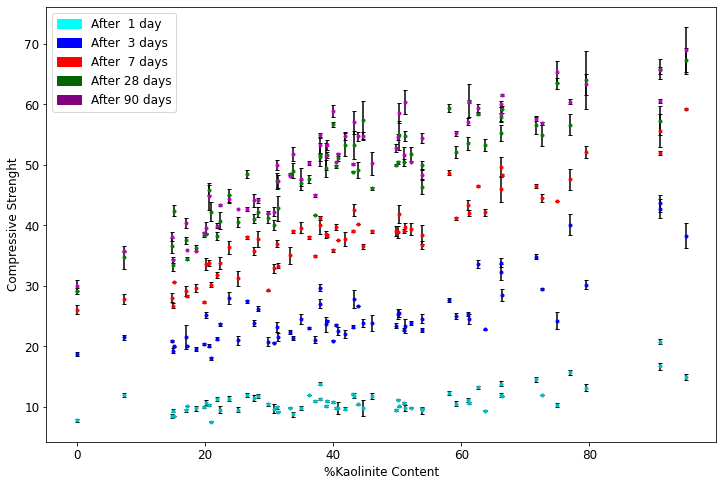
\includegraphics[width=\textwidth]{figures/cstrength-std.png}
  %\caption{Compressive strength in relation of Kaolinite content for days 1, 3 , 7, 28, 90 (each data-point was provided as a mean of 3 to 7 other samples we had not access to and its error-bars correspond to the standard deviation obtained for those means). }
  \vspace{-3mm}
  % TODO: When referencing it appears IV-A, can we put something more beautiful??
  \label{fig:kaolinite-cs}
\end{figure*}

\subsection{Outliers}
After visualizing the data, we appreciated a few possible outliers in the measurements at day 1 and 3. However, as all the experiments were repeated (in the laboratory at the EPFL, a reliable environment) and the behaviour was persistent we decided not to remove them. We did not remove either deviated pessimistic points since we are creating a model for construction materials and we considered more responsible to put ourselves in the worst case.


% KAOLINITE BASED MODELS
\section{Kaolinite-based models}

% Metrics for the model
% Linear     (for all the days)
% Non linear (for all the days)

Once detected the high correlation of the \textit{Kaolinite Content} with the compression strength for all the days contemplated. We decided to start creating simple models involving only this feature. %For these we established some metrics:

\subsection{R-squared and MSE}
R-squared is an almost perfect metric for knowing how good is our least squares model in this case. However, this metric is always improving as we add or create more variables to our regression so, for avoiding overfitting, we measure also the MSE of the model with leave one out cross validation which helps us to precisely estimate it with so little  data. 

\subsection{Linear Regression}
With this first approach we did not obtain good metrics for our models except for the day 7 model. This is because even when we know that there is a high correlation between \textit{Kaolinite Content} and compression strength, this relation has not to be linear. Visualizing the data it is reasonable clear that we need a model more expressive to better fit the data.

\subsection{Non Linear Models}
Following that logic, we used feature augmentation to add $\textit{Kaolinite Content Square}$ to our model so we can fit better the distribution of the data. This notably improved our models (specially for the days 28 and 90). We did not continue the feature augmentation (adding the cubic term) because visualizing the data it was clear that it followed a distribution increasing the compression strength when increasing the \textit{Kaolinite Content}. We wanted our model function to be increasing and considered not following having this behaviour a signal of overfitting.

It is precisely what happened in the models for days 1 and 3 where the parable vertex was inside of the range of the \textit{Kaolinite Content}. However, we could see that it was caused by the irregular data distribution in the feature domain.


% WARNING! This image is not fixed in it's position!!
\newpage
\begin{figure}
\begin{subfigure}{.5\textwidth}
  \centering
  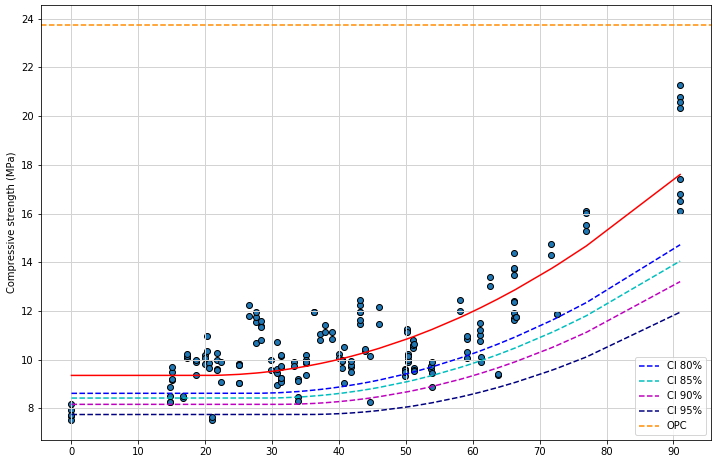
\includegraphics[width=0.84\columnwidth]{figures/day1_CI.png}
  \label{fig:sub-first}
\end{subfigure}
\newline
\begin{subfigure}{.5\textwidth}
  \centering
  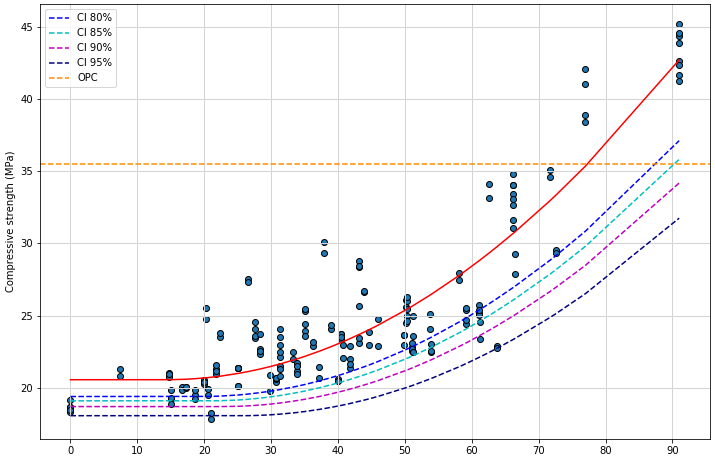
\includegraphics[width=0.84\columnwidth]{figures/day3_CI.png}
  \label{fig:sub-second}
\end{subfigure}
\newline
\begin{subfigure}{.5\textwidth}
  \centering
  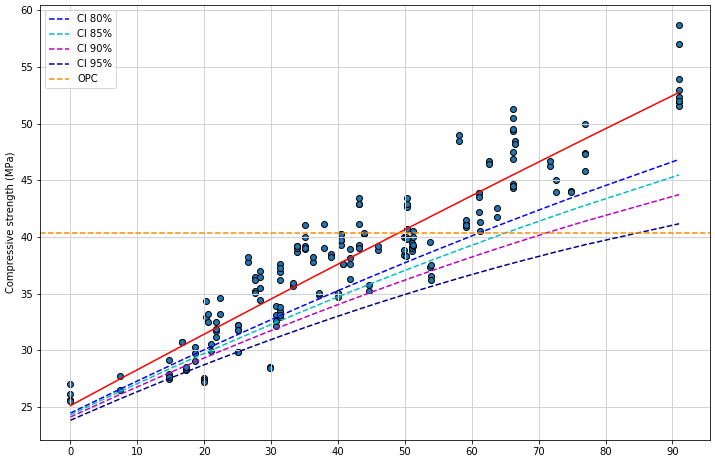
\includegraphics[width=0.84\columnwidth]{figures/day7_CI.png} 
  \label{fig:sub-third}
\end{subfigure}
\newline
\begin{subfigure}{.5\textwidth}
  \centering
  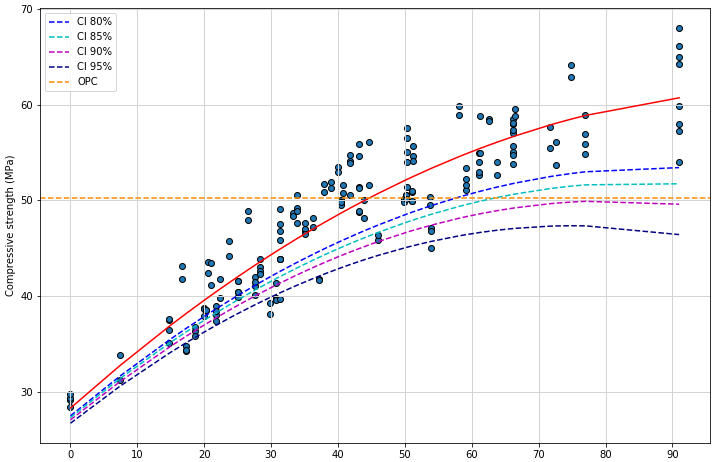
\includegraphics[width=0.84\columnwidth]{figures/day28_CI.png}  
  \label{fig:sub-fourth}
\end{subfigure}
\newline
\begin{subfigure}{.5\textwidth}
  \centering
  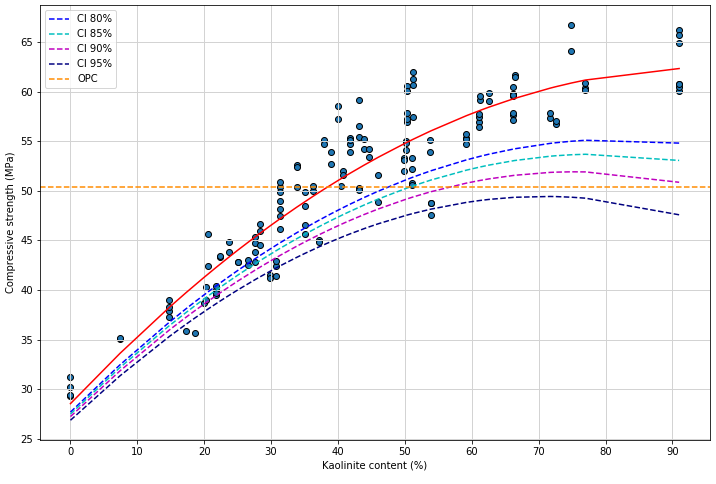
\includegraphics[width=0.84\columnwidth]{figures/day90_CI.png}  
  \label{fig:sub-fourth}
\end{subfigure}
\end{figure}

% CONFIDENCE ANALYSIS
\section{Confidence analysis}
% Explain
% Plot?

The little amount of data makes this even more important and, this part is also the one that justifies the effort for obtaining a full dataset (more points is what has given us smaller confidence intervals). We have created lower bounds of certain probabilities for the compressive strength of the LC3 depending on the \textit{Kaolinite Content} (graphics in the right, days 1 to 90 from up to down). 

These have been obtained with the python library \textit{statsmodels} and are confidence intervals for the linear regression parameters what, together with the fact that our points are not evenly distributed through all the \textit{Kaolinite Content} domain, could lead to certain parts of the model not having an accurate bound locally. We have not however appreciated this.



%\vspace{1cm}
% \begin{figure}[htbp]
%   \centering
%   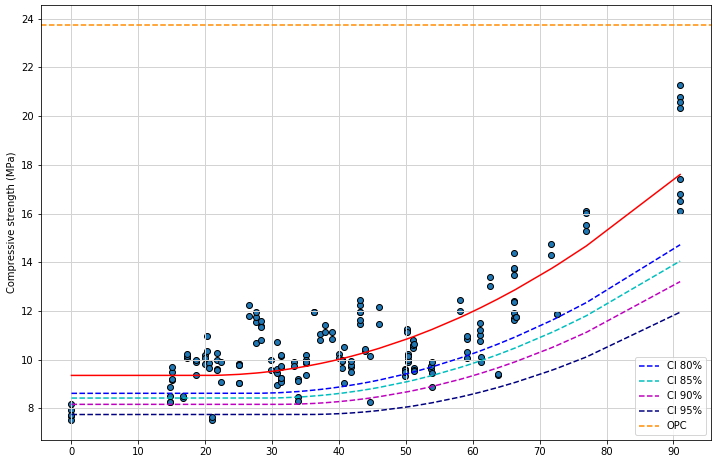
\includegraphics[width=0.8\columnwidth]{figures/day1_CI.png}
%   \vspace{-1.5cm}
%   \label{fig:denoise-wavelet}
% \end{figure}
% \begin{figure}[htbp]
%   \centering
%   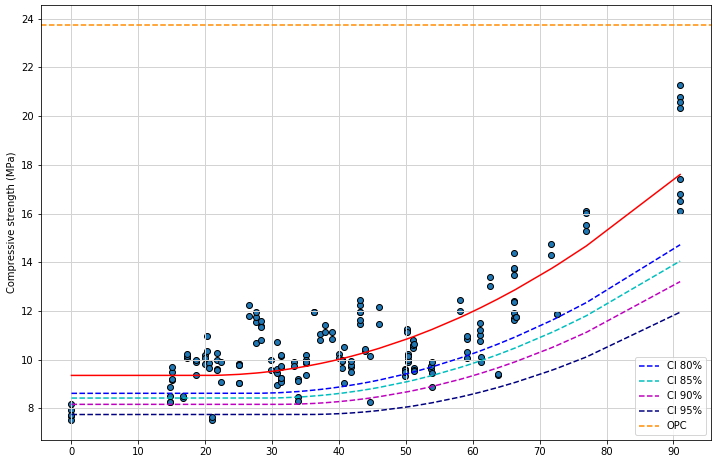
\includegraphics[width=0.8\columnwidth]{figures/day1_CI.png}
%   \vspace{-1.5cm}
%   \label{fig:denoise-wavelet}
% \end{figure}
% \begin{figure}[htbp]
%   \centering
%   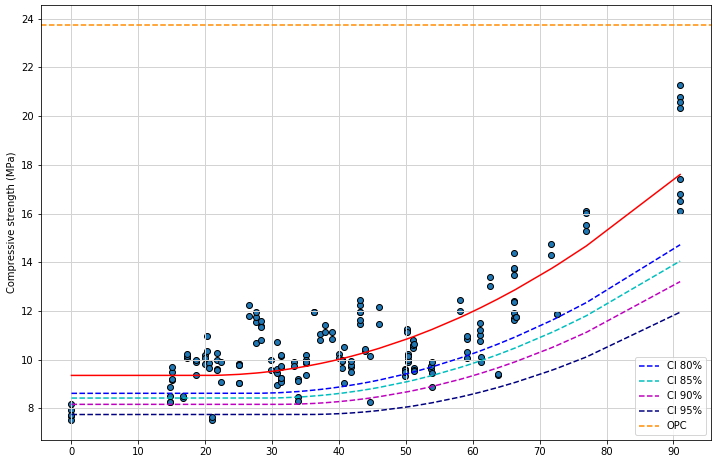
\includegraphics[width=0.8\columnwidth]{figures/day1_CI.png}
%   \vspace{-1.5cm}
%   \label{fig:denoise-wavelet}
% \end{figure}
% \begin{figure}[htbp]
%   \centering
%   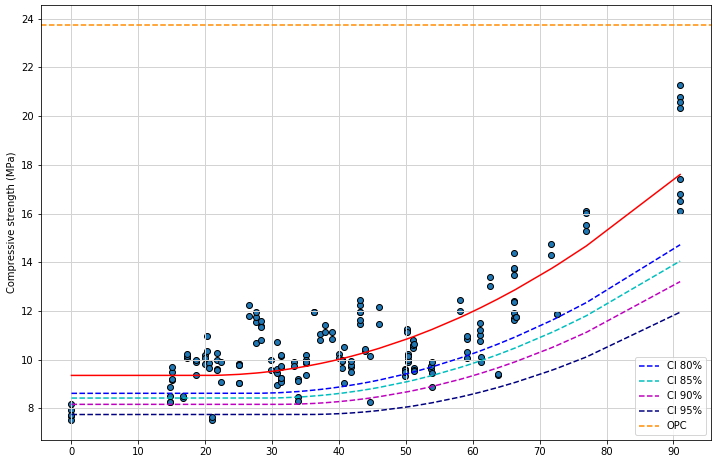
\includegraphics[width=0.8\columnwidth]{figures/day1_CI.png}
%   \vspace{-1.5cm}
%   \label{fig:denoise-wavelet}
% \end{figure}
% \begin{figure}[htbp]
%   \centering
%   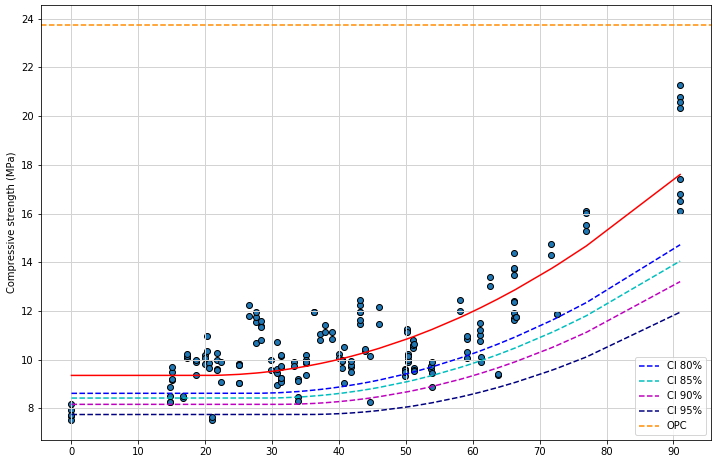
\includegraphics[width=0.8\columnwidth]{figures/day1_CI.png}
%   \vspace{-1.5cm}
%   \label{fig:denoise-wavelet}
% \end{figure}


% FEATURE SELECTION
\section{Feature selection}

% Adjusted R-squared
% MSE
% Leave one out

After creating the models based on the \textit{Kaolinite Content} we wanted to take advantage of these (and their shape, close to the data distribution) but reducing the points sparsification or distance to the model so we decided to add more features. Once again, we could not add many of them because it would lead to overfitting. We created a function to decide which features complemented best the Kaolinite-based model.

\subsection{Adjusted R-squared}
For deciding which was the best feature to be added to our model we used adjusted R-squared. It is a version R-squared adjusted for the number of predictors in the model. The adjusted R-squared increases only if the new term improves the model more than what would be expected by chance. It can decrease otherwise. Since in our case we only had a few points, it provided us with a way to penalize equations that take into account many variables, helping us to avoid overfitting. As always, we also considered MSE computed with leave one out cross validation for avoiding overfitting.

\subsection{Relevant features}
Since most of the features had missing values and this translated into dropped points, we realized that some features were having a bigger adjusted R-squared because after dropping missing values they had few points remaining (and of course it is easier to fit better less points with the same number of variables). We could not trust these features but it let us see their potential. We set a threshold for relying the features and got that the most relevant features were (ordered by relevance and reliability):
\textit{BET\_specific\_surface, span, D90, D10}
% \begin{itemize}
%     \item BET\_specific\_surface
%     \item span
%     \item D90
%     \item D10
%\end{itemize}

That is, the ones related with the size and shape of the particles in the clay are more relevant than those of the chemical composition (leaving aside the \textit{Kaolinite Content}).

% MULTIPARAMETER MODELS
\section{Multiparameter models}
Continuing with this approach, and taking into account the reliable features, we improved the kaolinite-based models by adding these features.

% Please add the following required packages to your document preamble:
\vspace{-2mm}
\begin{table}[h]
\centering
\resizebox{\columnwidth}{!}{%
\begin{tabular}{l|l|l|l|l|l|l|l|l|}
\cline{2-9}
                                                & Intercept & Kaolinite & Kaolinite\textasciicircum{}2 & D10     & D90    & SPAN   & BET     & adjusted R2 \\ \hline
\multicolumn{1}{|l|}{\multirow{5}{*}{Day 1}}    & 9,9983    & -0,0649   & 0,0016                       &         &        &        &         & 0,7051      \\ \cline{2-9} 
\multicolumn{1}{|l|}{}                          & 0,1622    & -0,3757   & 0,9814                       & -0,0564 &        &        &         & 0,8080      \\ \cline{2-9} 
\multicolumn{1}{|l|}{}                          & 0,1324    & -0,3595   & 0,9952                       &         & 0,0369 &        &         & 0,8040      \\ \cline{2-9} 
\multicolumn{1}{|l|}{}                          & 0,1494    & -0,3938   & 0,9675                       &         &        & 0,0573 &         & 0,7052      \\ \cline{2-9} 
\multicolumn{1}{|l|}{}                          & 0,1445    & -0,2789   & 0,8748                       &         &        &        & -0,0063 & 0,7300      \\ \hline
\multicolumn{1}{|l|}{\multirow{5}{*}{Day   3}}  & 21,3410   & -0,1077   & 0,0038                       &         &        &        &         & 0,8159      \\ \cline{2-9} 
\multicolumn{1}{|l|}{}                          & 0,1221    & -0,3282   & 1,1413                       & -0,0881 &        &        &         & 0,8900      \\ \cline{2-9} 
\multicolumn{1}{|l|}{}                          & 0,0646    & -0,3333   & 1,2087                       &         & 0,1321 &        &         & 0,8970      \\ \cline{2-9} 
\multicolumn{1}{|l|}{}                          & 0,1150    & -0,5741   & 1,3381                       &         &        & 0,1874 &         & 0,7052      \\ \cline{2-9} 
\multicolumn{1}{|l|}{}                          & 0,1169    & -0,2869   & 1,0961                       &         &        &        & -0,0236 & 0,7052      \\ \hline
\multicolumn{1}{|l|}{\multirow{5}{*}{Day   7}}  & 25,1080   & 0,3188    & -0,0002                      &         &        &        &         & 0,8566      \\ \cline{2-9} 
\multicolumn{1}{|l|}{}                          & 0,0066    & 0,8585    & -0,0326                      & 0,0106  &        &        &         & 0,8930      \\ \cline{2-9} 
\multicolumn{1}{|l|}{}                          & -0,0106   & 0,8371    & 0,0121                       &         & 0,0959 &        &         & 0,9060      \\ \cline{2-9} 
\multicolumn{1}{|l|}{}                          & 0,0051    & 0,6844    & 0,1133                       &         &        & 0,1333 &         & 0,8850      \\ \cline{2-9} 
\multicolumn{1}{|l|}{}                          & 0,0079    & 0,8748    & -0,0499                      &         &        &        & -0,0133 & 0,8820      \\ \hline
\multicolumn{1}{|l|}{\multirow{5}{*}{Day   28}} & 28,3029   & 0,6215    & -0,0029                      &         &        &        &         & 0,8459      \\ \cline{2-9} 
\multicolumn{1}{|l|}{}                          & -0,0204   & 1,4722    & -0,6379                      & 0,0261  &        &        &         & 0,8820      \\ \cline{2-9} 
\multicolumn{1}{|l|}{}                          & -0,0253   & 1,4543    & -0,6107                      &         & 0,0665 &        &         & 0,8870      \\ \cline{2-9} 
\multicolumn{1}{|l|}{}                          & 0,0192    & 1,3059    & -0,5294                      &         &        & 0,0597 &         & 0,8350      \\ \cline{2-9} 
\multicolumn{1}{|l|}{}                          & 0,0095    & 1,4970    & -0,6937                      &         &        &        & -0,0344 & 0,8560      \\ \hline
\multicolumn{1}{|l|}{\multirow{5}{*}{Day   90}} & 28,5634   & 0,7116    & -0,0037                      &         &        &        &         & 0,8654      \\ \cline{2-9} 
\multicolumn{1}{|l|}{}                          & -0,0276   & 1,8278    & -0,9080                      & 0,0113  &        &        &         & 0,9010      \\ \cline{2-9} 
\multicolumn{1}{|l|}{}                          & -0,0291   & 1,8216    & -0,8984                      &         & 0,0249 &        &         & 0,9020      \\ \cline{2-9} 
\multicolumn{1}{|l|}{}                          & -0,0098   & 1,7392    & -0,8471                      &         &        & 0,0006 &         & 0,7052      \\ \cline{2-9} 
\multicolumn{1}{|l|}{}                          & -0,0202   & 1,8481    & -0,9367                      &         &        &        & -0,0326 & 0,8880      \\ \hline
\end{tabular}%
}
\end{table}
\vspace{-2mm}
%M Explain the lack of features that seemed importants (reliable data)
% Board with parameters/confidence intervals for these models
% Add confidence intervals
% Explain that ridge regression didn't work for us


% TODO: It's not deleted! take from here what you consider!
% \newpage
% % MODELS AND METHODS
% \section{Models and methods}
% \subsection{Linear Regression}
% \subsubsection{Ordinary Least Squares}
% We started with simple models, using ordinary least squares to obtain the relation between compressive strength and kaolinite level, which was the feature with the best performance.
% \subsubsection{Weighted Least Squares}
% % \begin{figure*}[tbp]
% %   \centering
% %   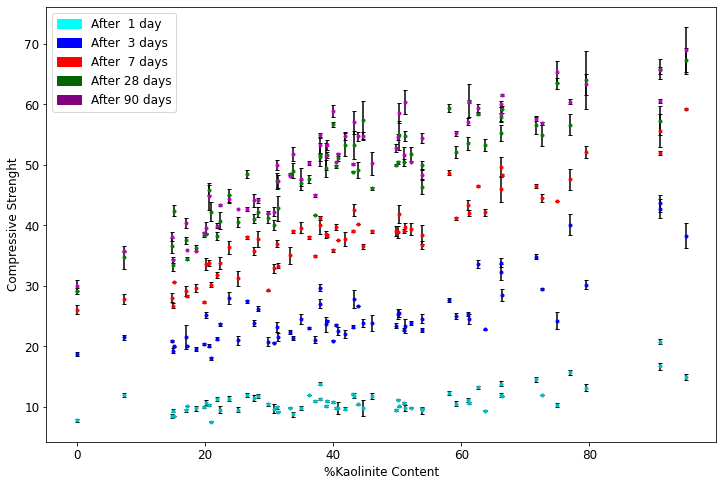
\includegraphics[width=\textwidth]{figures/cstrength-std.png}
% %   \caption{Compressive strength in relation of Kaolinite content for days 1, 3 , 7, 28, 90 (each data-point was provided as a mean of 3 to 7 other samples we had not access to and its error-bars correspond to the standard deviation obtained for those means). }
% %   \vspace{-3mm}
% %   \label{fig:cstrength-std}
% % \end{figure*}
% Data provided us with a standard deviation for each mean (datapoint for compressive strength) [Figure~\ref{fig:denoise-wavelet}], so we decided to carry out another approach: modeling the data weighting these means with their standard deviation. We had to come up with a way to model our data in which the larger the standard deviation was, the less importance the sample had to have. 
% To do this, we opted to use a tailor-made version of the method the WLS (Weighted Least Squares) provided by the \textit{statsmodels} library \cite{sm:wls}. \textit{The weighted least squares method is a generalization of the ordinary least squares and linear regression in which the errors covariance matrix is allowed to be different from an identity matrix [...]}

% \textit{If the errors are uncorrelated and have equal variance, then the minimum of the function}
% \newline
% $
% S({\boldsymbol{\beta }})=\sum_{i}{r_{i}({\boldsymbol{\beta }})^{2}}
% $,
% \textit{is found when}
% $
% \displaystyle{\frac{\partial S({\hat {\boldsymbol {\beta }}})}{\partial \beta _{j}}}=0
% $
% \textit{(defining ${\displaystyle {\boldsymbol {\hat {\beta }}}}$). }
% \newline
% \newline
% \textit{[...] The Gauss–Markov theorem shows that, when this is so, Beta is a "best linear unbiased estimator" (BLUE). If, however, the measurements are uncorrelated but have different uncertainties, a modified approach might be adopted. Aitken showed that when a weighted sum of squared residuals is minimized, Beta is the BLUE if each weight is equal to the reciprocal of the variance of the measurement.}\cite{wiki:wls}

% So the usual way to use this method is to provide the reciprocal of the variance of the measurement. That is, concerning the rest of the samples. As in our case, the data samples had their standard deviation,  one way to introduce this variance in our model would be to take the current value of the variance of each sample concerning its partners and multiply it by the standard deviation provided squared. And so, obtaining the weights that would give us the BLUE. 

% To simplify, for this report we limit ourselves to a modified approach in which we normalize the standard deviations given and input the inverse value to our \textit{statsmodels} module.

% \subsection{Non Linear Models}
% Continuing with that approach, and adding a little more complexity, we have used feature augmentation, and we have done the regression with kaolinite, kaolinite square and another variable. We have chosen to make feature augmentation of the Kaolinite because it is the feature that has the greatest relationship to compressive strength, as we have seen in the correlation analysis as in the MSE and R2 analysis.  And then based on these analyses we have selected another feature that will allow us to improve the model.
% \subsection{Confidence Intervals}
% The objective of this method is to provide a more mathematical analysis of the confidence we can expect from our models, and give a better answer to the questions the lab wants our model to answer. This applies to the models used with and without the standard deviation given

\section{STANDARD DEVIATION}

Finally, we created models taking into account the standard deviation by applying a tailor-made version of the Weighted Least Squares method provided by the StatsModels library [11, 12]. The ideal weight is the inverse of the variance of the measurements (more importance is given to the samples with less variability), this is the approach we utilized but it required removing certain points coming from the execution of a single experiment and therefore with standard deviation zero. 

We appreciated that the models for later days were more stable and less influenced by this weighted approach than those for earlier days.

\begin{figure}[htbp]
  \centering
  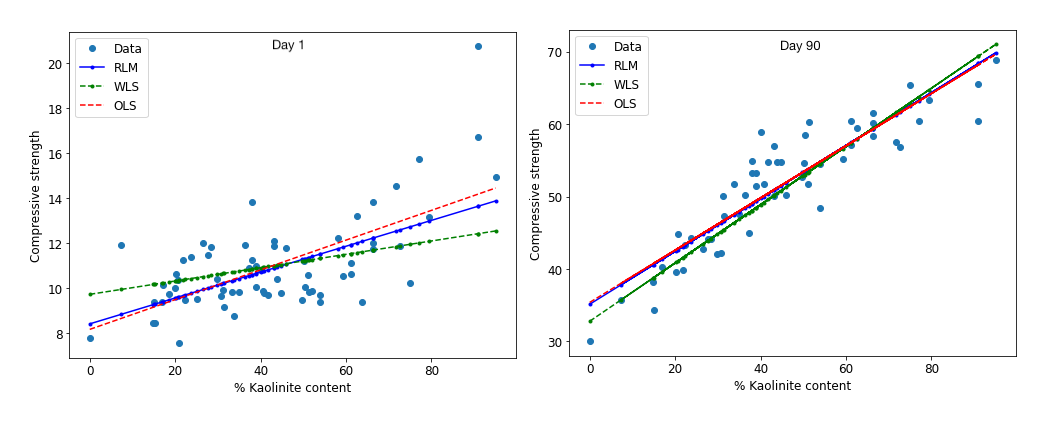
\includegraphics[width=\columnwidth]{figures/lr-ols-wls-rls-d1-d90.png}
  \vspace{-3mm}
  \caption{Weighted Least Squares, Ordinary Least Squares, and Recursive Least Squares models for days 1 and 90}
  \label{fig:wls-comp}
\end{figure}

After analyzing more in detail the models we observed that another very determining factor for the construction of a method such as this was also to take into account the number of samples that have been used to calculate each mean, since a mean in which only one sample has been used would have a zero standard deviation and yet is a much less reliable sample. Furthermore, for our model to achieve something close to the Best Least Unbiased Estimator (BLUE), many tests or researches were required.

Finally, we analyzed the standard deviation as a function of time to see if the different curve trends obtained in our data are dependent on the days. We obtain a slightly increasing trend until the 27th and it goes down again for the 90th. This is to be expected as with each passing day it is more likely that over time the conditions that each piece of cement analyzed has received are more likely to have been different. However, it is reduced on the last day (day 90) as at this point the cement samples to be tested have been reduced, so the measurements here are a little less reliable.

\begin{figure}[htbp]
  \centering
  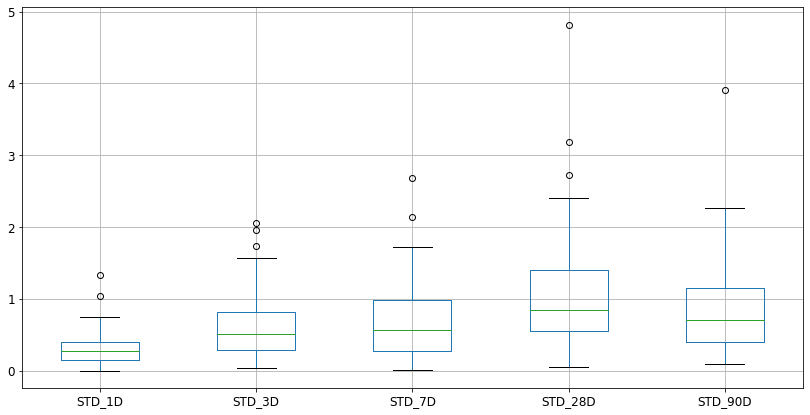
\includegraphics[width=\columnwidth]{figures/stds-days.png}
  \vspace{-3mm}
  \caption{Standard deviations days 1, 3, 7, 28, and 90}
  \label{fig:stds-days}
\end{figure}



\section{Conclusions}
\begin{itemize}
\item The scarcity of data has made us opt for simple models, but which in turn can answer the questions posed to us from the laboratory.

\item Kaolinite content has a strong relationship to compressive strength.
\item On days 1 and 3 we see a little more random behaviour and a worse performance than in the case of using normal cement, but from day 7 we see a much more stable behaviour. This may be due to the setting time. This is why we consider that it makes more sense to work with the data from the first week, when studying the behavior of clays and making decisions about which clay to use.
\item On the 28th and 90th days, we clearly see how for low values of Kaolinite, there is a linear relationship with the compressive strength but for intermediate and high values of Kaolinite the compressive strength tends to stabilise at one value, so the non-linear model is best suited to the data.
\item LC3 is a solid alternative to the classical cement in terms of mechanical properties for clays with \textit{Kaolinite Content} greater or equal than 50\%. 
\end{itemize}


\section*{Acknowledgements}

Our deepest thanks to Franco Zunino for allowing us to contribute to this project and help us throughout the process.

We also want to express our gratitude to the Complutense and the Polytechnic Universities of Madrid as well as to the EPFL for all the knowledge and opportunities offered.

\newpage
\nocite{*}
\bibliographystyle{IEEEtran}
\bibliography{literature.bib}

\end{document}
